\documentclass[12pt, twoside]{article}
\usepackage[hmargin=1.25in, vmargin=1.1in]{geometry}

\usepackage[utf8]{inputenc}
\usepackage[T1]{fontenc}
\usepackage[english]{babel}
\usepackage{pdfpages}
\usepackage{listings}
\usepackage{color}
\usepackage{graphicx}
\usepackage{float}
\usepackage{hyperref}
\usepackage{url}
\usepackage{upquote}
\usepackage{lastpage}
\usepackage{fancyhdr}
\pagestyle{fancy}
\usepackage{longtable}
\usepackage{tabu}
\usepackage{rotating}
\usepackage[strings]{underscore}
\usepackage[nottoc,numbib]{tocbibind}

\graphicspath{ {images/} }

\newcommand{\helv}{\fontfamily{phv}\fontseries{b}\fontsize{9}{11}\selectfont}

%--------------- Variables à modifier à chaque rendu ---------------
\title{Specifications}
\newcommand{\daterendu}{05/31/2019}
%-------------------------------------------------------------------

\makeatletter\let\Title\@title\makeatother

% Décommenter pour commencer les chapitres à 0
%\setcounter{section}{-1}

\begin{document}

\begin{titlepage}

\newcommand{\HRule}{\rule{\linewidth}{0.5mm}} % Defines a new command for the horizontal lines, change thickness here

\center % Center everything on the page



\includegraphics[width=0.8\textwidth]{logo_HEIA.jpg}

\includegraphics[width=0.3\textwidth]{logo_LBNL.png}\\[1.1cm]
\textsc{\Large Bachelor thesis \\ [0.3cm]
\large Year 2018-2019 }\\ [2.0cm]


\textsc{
\bfseries \LARGE Machine learning for noise reduction in images of old audio records}\\ [1.0cm]


\HRule \\[0.5cm]
{ \huge \bfseries \Title }\\ 
\HRule \\[1.2cm]

\Large
Benoit \textsc{Ruffray}\\[1.0cm] 

{\large Date : \daterendu}\\[1.3cm] 

\begin{flushleft}
\large External supervisor: Haber~Carl
\end{flushleft}
\begin{flushleft}
	\large Internal supervisors: Bapst~Frédéric / Hennebert~Jean
\end{flushleft}
\begin{flushleft}
\large Consultants: Cornell~Earl / Nachman~Benjamin
\end{flushleft}

\end{titlepage}
\pagenumbering{Roman}

\renewcommand{\headrulewidth}{1pt}
\fancyhead[L]{\helv ML-for-NR}
\fancyhead[C]{\helv 2018-2019}
\fancyhead[R]{\helv \Title }

\renewcommand{\footrulewidth}{1pt}
\fancyfoot[C]{\helv Table of contents \thepage{}}

\setcounter{page}{1}

\begin{center}
\tableofcontents
\end{center}

\newpage

\fancyhf{}
\renewcommand{\headrulewidth}{1pt}
\fancyhead[L]{\helv ML-for-NR}
\fancyhead[C]{\helv 2018-2019}
\fancyhead[R]{\helv \Title }

\renewcommand{\footrulewidth}{1pt}
\fancyfoot[LO, RE]{\helv Bachelor thesis, year 2018 - 2019}
\fancyfoot[C]{}
\fancyfoot[RO, LE]{\helv \textbf{Page \thepage{}/\pageref{LastPage}}}
\pagenumbering{arabic}
\setcounter{page}{1}
\section{Introduction}
This document specifies the context and objectives of the Bachelor project "Machine learning for noise reduction in images of old audio records". This project is done under the supervision of Mr. Carl Haber at the Lawrence Berkeley National Laboratory, and supervised by Messrs. Frédéric Bapst and Jean Hennebert at the University of Applied Science of Fribourg.
\section{Context}
"Machine learning for noise reduction in images of old audio records" (ML4NR) is a project proposed by Mr. Carl Haber at the Lawrence Berkeley National Laboratory (LBNL). It is part of a project for the Library of Congress, whose goal is the restoration and conservation of old audio records.
ML4NR is done as a Bachelor Thesis project by Mr. Benoît Ruffray.
\subsection{Mechanical Audio records}
The first device able to record and play back sound waves was an invention of Thomas Edison in 1877, the cylinder phonograph\cite{audio}. This device could record sounds by making a needle vibrate and carve a groove on a rotating tinfoil or wax cylinder. To play it back, the cylinder was rotated, making the needle vibrate while following the groove. This vibration is amplified and produces audible sound waves, the ones recorded.

Since cylinders were impractical to store and quick to be damaged (the physical contact would wear out the groove after each play), Emile Berliner improved the concept in 1887 by inventing a flat support for audio recording, discs. Those were easier to stack and reproduce, and so quickly overtook the market. The associated device is the gramophone.

The standard format from the 1910s to 1950s was a double-sided 78 rpm shellac disc. However, shellac is a brittle material, and the hard needles would wear them out quickly. It's in 1948 that Columbia Records invented the 33 rpm vinyl disc. Vinyl is more expensive but sturdier than shellac, and the longer playtime would compensate for the extra cost. RCA Victor introduced the 45 rpm, smaller vinyl disc in 1949, effectively cutting the cost by using less material. Both formats replaced the shellac disc.

The Library of Congress is interested in the conservation of these old records, as they contain valuable historical audio data such as presidential speeches, native American interviews, or traditional songs from the past. However, since the cylinders and shellac discs are getting destroyed with each play, they associated with the LBNL to find a way to extract and preserve all data without physical contact (non invasive play back). They came up with the IRENE system.
\subsection{IRENE and Weaver}
IRENE is a system that can image any kind of engraved support using high definition cameras. One picture is a really thin line across the entire support, and a lot of them are taken while the record is moved.

It shines light in a certain direction towards the record to obtain a black and white picture: the white part is the light reflected to the camera, the black part isn't. For shellac discs, white parts are flat, black ones are inclined. This helps finding the groove, as its bottom is flat.
\begin{figure}[H]
	\centering
	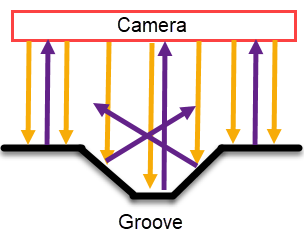
\includegraphics[width=0.5\textwidth]{grooveside.png}
	\caption{Camera lighting the groove and detecting direct reflection}
	\label{grooveside}
\end{figure}
\begin{figure}[H]
	\centering
	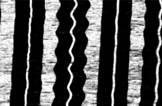
\includegraphics[width=0.5\textwidth]{groove.png}
	\caption{Resulting image of grooves}
	\label{groove}
\end{figure}
Any kind of damage or unwanted object on the disc can be seen, as it disturbs direct reflection. It is considered as noise on the image. A shellac disc imaged entirely takes multiple gigabytes of space.

Along with this system exists a program named Weaver, made in C\#. It is a collection of plugin developed through the years by researchers and students, and is used to pipeline the data reading process. Weaver's main function is to generate the sound wave from the imaged grooves, using an edge detection algorithm to find the exact center of the groove. However, since the images are noisy (dust, damage), the sound generated also contains a high frequency background noise. Simply cutting the high frequencies wouldn't completely work, as the noise in images can also influence lower frequencies.
\subsection{Machine learning}
Machine learning is a powerful computing technique used for handling problems having too much features for a deterministic algorithm. For example, object detection and classification in pictures or market predictions.

It is based on multiple layers of neurons. Each layer takes some data as input, does some transformation, and feeds the output to the next layer. By setting a goal (ground-truth), it can evaluate its result, and change slightly the transformations occurring in all layers (weight adjustment). It repeats this process over and over until satisfied.
\section{Objectives}
The main goal of the ML4NR project is to generate a cleaner sound than the deterministic algorithm when given noisy groove images as input, using machine learning. Since it was never attempted before at the LBNL, the project is divided into steps, which correspond to working prototypes.
\subsection{Prototype 0}
This prototype serves as training for using KERAS. It'll teach the basics of model building. It's goal is to have a result on the MNIST dataset (not necessarily good). 
\subsection{Prototype 1}
This prototype is a proof of concept. Using Weaver, groove images of pure sine waves are generated. They are used to train a model, whose goal will be to find the simple frequency sound wave from the image. A metric needs to be defined for result evaluation.
\subsection{Weaver Plugin}
The Weaver plugin needs to be modified, in order for it to be able to generate noisy groove images. The artificial noise needs to have the same properties as the real one (in actual imaged grooves).
\subsection{Prototype 2}
This prototype tests the robustness of the model built before. It uses the noisy groove images generated with the Weaver plugin as input, and tries to find the clear sound wave. SOTA analysis helps improvement of the model.
\subsection{Prototype 3}
This prototype checks if complex sound waves can be generated by the model. Actual images of discs are used as input, and the goal is to find the same sound that is generated using the deterministic algorithm. Maybe a "bad result" regarding the goal could be better than current results.
\subsection{Prototype 4}
Final prototype, it uses the actual images of the discs, and the corresponding clean sound as goal. The clean sound is either obtained from a recorded stylus play, of from the original audio tape (which was used to print the disc). The results of this prototype are the results of the project.

If needed, this prototype is implemented as a plugin in Weaver.  
\section{Tasks}
\subsection{Prototype 0}
\begin{description}
	%	\item[n] d
	\item[Familiarize with KERAS and TensorFlow] Read documentation and set up a working environment for KERAS. Learn how to use.
	 \item[Analyze layer types] Read about the types of layer commonly used when building a machine learning model. Find specific ones for this context.
	 \item[Build own model] Create a model that can deal with pattern recognition, for handwritten characters.
	 \item[Train and test on MNIST dataset] Train model on MNIST dataset (handwritten numbers) and test accuracy/precision. No need to have good results, it is a proof of concept.
\end{description}
\subsection{Prototype 1}
\begin{description}
	%	\item[n] d
	\item[Analyze SOTA of sound generation] Analyze the current State of the Art in sound generation using machine learning.
	\item[Define a metric for model evaluation] Define which metric should be used to determine if a model is good or not.
	\item[Documentation of SOTA] Produce a written document on current SOTA, for future use.
	\item[Familiarize with Weaver] Learn how to use Weaver, the pipelining tool for IRENE.
	\item[Generate dataset of sine grooves] Use Weaver to generate a dataset of groove images whose base is a simple sine wave (one single frequency). The groove should be clean.
	\item[Create or use model for sound generation from images] Based on the SOTA, create or use a model able to generate sound from groove images.
	\item[Train and test model] Train the model with the dataset previously generated.  Use pure single frequency sound as ground-truth. Test with metric defined earlier. Improve the model and parameters to have better results.
	\item[Documentation of prototype] Document everything about the prototype, from researches to code comments.
\end{description}
\subsection{Weaver Plugin}
\begin{description}
	%	\item[n] d
	\item[Familiarize with plugin code] Read and understand the code of the Weaver groove image generator plugin.
	\item[Analyze structure and properties of noise] Analyze all the properties of actual discs images noise.
	\item[Implement modified plugin to generate noisy grooves] Modify the plugin so it can generate noisy grooves, with a noise having the same properties as actual discs images.
	\item[Document new plugin] Document everything used for this plugin, as well as noise properties.
\end{description}
\subsection{Prototype 2}
\begin{description}
	%	\item[n] d
	\item[Generate dataset of noisy sine grooves] Use previously implemented plugin to generate a dataset of images with grooves of simple sine waves, but noisy.
	\item[Train and test previous model] Try to train previous model with noisy images, and see what it can do. Use pure single frequency sound as ground-truth (not noisy sound). Use the metrics defined.
	\item[Analyze SOTA and leads to improve model] Use SOTA documentation and leads from workshops to improve the model and the results, regarding the metrics.
	\item[Document prototype] Document everything about the prototype, from researches to code comments.
\end{description}
\subsection{Prototype 3}
\begin{description}
	%	\item[n] d
	\item[Obtain dataset of imaged discs and generated sound] Obtain dataset of actual noisy grooves, imaged by IRENE, and their corresponding sound generated with Weaver.
	\item[Train and test previous model] Use model made for simple frequencies and test results. See if it can find the actual sound. The ground-truth is the noisy sound generated by Weaver.
	\item[Improve model with leads and SOTA] Check documentation and leads, improve model and parameters until it obtains a good result regarding the metrics.
	\item[Document prototype] Document everything about the prototype, from researches to code comments. 
\end{description}
\subsection{Prototype 4}
\begin{description}
%	\item[n] d
    \item[Obtain dataset of imaged discs and recorded sound] Obtain dataset of actual noisy grooves, imaged by IRENE, and their corresponding sound recorded when played with a stylus. The sound could also come from the original tape.
    \item[Train and test previous model] Use model made previously and test results. See if it can find the actual sound. The ground-truth is the clean sound obtained by stylus play or from the original tape.
    \item[Improve as much as possible] Check documentation and leads, improve model and parameters until it obtains a good result regarding the metrics.
    \item[Document prototype] Document everything about the prototype, from researches to code comments. 
\end{description}
\subsection{Integration to Weaver}
\begin{description}
	%	\item[n] d
	\item[Adapt code, I/O, to integrate with Weaver] If necessary, find a way to implement the model in a Weaver plugin, so it can be used for pipelining.
	\item[Document how to use] Document the plugin code and its usage.
\end{description}
\subsection{Documentation and administration}
In addition to prototypes documentation, the final report should be written along the project. A work journal should be maintained regularly, and weekly meetings held with the supervisors. All decisions and discussions should be written in minutes. All written documents are shared with the supervisors and experts on the designated platform.

\section{Planning}
See end of document.
\bibliographystyle{unsrt}
\bibliography{cdc}
\includepdf[pages={3}]{planV1.pdf}
\end{document}